\chapter{HTTP, API, REST}
\section{HTTP}
	Protokół HTTP (Hypertext Transfer Protocol) jest fundamentem, na którym postawiona jest współczesna komunikacja w internecie. HTTP działa w architekturze klient-serwer co oznacza, że zapytania, inicjowane przez odbiorcę (najczęściej przeglądarkę internetową), wysyłane są do serwera, a ten zwraca określoną odpowiedź. W celu wyświetlenia strony internetowej przeglądarka wysyła żądanie pobrania dokumentu HTML, który reprezentuje stronę WWW. Następnie przeglądarka analizuje otrzymany plik, wykonuje dodatkowe żądania w celu uzyskania informacji na temat układu strony (CSS) i pobrania podzasobów zawartych na stronie (obrazki, filmy video). Przeglądarka łączy wszystkie otrzymane w ten sposób zasoby, aby zaprezentować kompletny dokument - stronę WWW. Skrypty wykonywane przez przeglądarkę mogą pobierać kolejne zasoby w późniejszych fazach, a ta na bieżąco aktualizuje stronę \cite{MozillaHTTP}.

	\subsection{Własności HTTP}
		\begin{enumerate}
			\item niezależny od typów danych - każdy typ danych może być przesyłany za pomocą HTTP, o ile zarówno klient, jak i serwer wiedzą, jak je obsłużyć. Wymagane jest, aby zarówno klient, jak i serwer określili typ zawartości za pomocą odpowiedniego typu MIME (Multipurpose Internet Mail Extensions - standard, który wskazuje, jaki rodzaj dokumentu, pliku lub strumienia bajtów jest przesyłany).
			
			\item rozszerzalny - nagłówki HTTP pozwalają w łatwy sposób dodać nowe parametry do protokołu. Należy jedynie ustalić semantykę nowego nagłówka między klientem a serwerem. Niestandardowe nagłówki wykorzystuje się w celu przesyłania dodatkowych danych na temat żądań i odpowiedzi.
			
			\item bezstanowy, ale nie bez sesji - serwer i klient są świadomi siebie nawzajem tylko podczas bieżącego żądania. Oznacza to, że nie ma powiązania między dwoma żądaniami wykonywanymi kolejno przez tego samego klienta. Dla użytkowników, którzy chcą w ciągły sposób wchodzić w interakcję z niektórymi stronami (np. poruszać się jako zalogowany użytkownik po aplikacji e-learningowej), może stanowić do duży problem. Jednym z rozwiązań tego problemu są ciasteczka HTTP. Te pozwalają na stworzenie sesji dla każdego zapytania w celu udostępnienie tego samego kontekstu lub stanu.
			
			\item niezawodny - protokół powinien być niezawodny, przesyłane wiadomości nie mogą być tracone. Wśród dwóch najpopularniejszych protokołów służących do transportowania danych w internecie (TCP/UDP) TCP jest niezawodny. Oznacza to, że sam protokół posiada mechanizmy sprawdzające, czy wszystko, co zostało przesłane, dotarło do odbiorcy i właśnie z tego powodu HTTP oparty jest na standardzie TCP.
		\end{enumerate}
	
	\subsection{HTTPS}
		Połączenia z wykorzystaniem protokołu HTTP nie są szyfrowane. Oznacza to, że dane wysyłane przez klienta nie są chronione, w szczególności poufne dane, takie jak hasła. Strony, które opierają swoją komunikację o HTTP, nie są bezpieczne dla użytkowników i odchodzi się od nich na rzecz HTTPS.
		
		HTTPS (Hypertext Transfer Protocol Secure) to rozszerzenie HTTP, które wykorzystywane jest do bezpiecznej komunikacji w internecie. Protokół komunikacji jest szyfrowany przy pomocy Transport Layer Security (TLS) lub wcześniej Secure Sockets Layer (SSL) \cite{WikipediaHTTPS}.
		
		HTTPS tworzy bezpieczny kanał, który chroni przed atakami podsłuchującymi i atakami typu "man-in-the-middle", pod warunkiem, że stosowane są odpowiednie pakiety szyfrowania, a certyfikat serwera jest zaufany i zweryfikowany.
	
	\subsection{Metody HTTP}
		HTTP definiuje dziewięć metod, które pozwalają określić jaka akcja powinna zostać wykonana dla określonego zasobu \cite{MozillaHTTPMethods}.
		
		\begin{itemize}
			\item GET - żąda reprezentacji określonego zasobu. Żądania używające metody GET powinny być wykorzystywane jedynie do pobierania danych \cite{RESTfulWebServices}.
			\item HEAD - żąda takiej samej odpowiedzi jak GET, ale bez treści odpowiedzi (response body).
			\item POST - wysyła dane do serwera, najczęściej w celu stworzenia zasobu.
			\item PUT - wysyła dane do serwera w celu zastąpienia zasobu nową reprezentacją.
			\item PATCH - wysyła dane do serwera w celu częściowej aktualizacji zasobu.
			\item DELETE - usuwa określony zasób.
			\item CONNECT - ustanawia tunel do serwera.
			\item OPTIONS - opisuje możliwości komunikacji.
			\item TRACE - wykonuje test zwrotny do zasobu docelowego.
		\end{itemize}
		
	\subsection{Kody odpowiedzi HTTP}
		Kod odpowiedzi HTTP informuje użytkownika o statusie żądania HTTP. Kody są podzielone na pięć grup: \cite{MozillaHTTPStatuses}
		\begin{enumerate}
			\item kody informacyjne (100 - 199)
			\item kody powodzenia (200 - 299)
			\item kody przekierowania (300 - 399)
			\item kody błędu aplikacji klienta (400 - 499)
			\item kody błędu aplikacji serwera (500 - 599)
		\end{enumerate}
		Powyższe kody odpowiedzi są zdefiniowane przez \href{https://httpwg.org/specs/rfc9110.html#overview.of.status.codes}{RFC 9110}. Popularne kody odpowiedzi:
		\begin{itemize}
			\item 200 OK - zapytanie się powiodło.
			\item 201 Created - zapytanie powiodło się i powstał nowy zasób.
			\item 204 No Content - zapytanie powiodło się, ale nie ma dla niego treści odpowiedzi.
			\item 301 Moved Permanently - URL zasobu zmieniło się na stałe. Nowe URL jest podawane w odpowiedzi.
			\item 302 Found - zasób został odnaleziony, jednak nie w miejscu, w którym go oczekiwano.
			\item 400 Bad Request - serwer nie obsłuży zapytanie z powodu błędu w zapytaniu klienta.
			\item 401 Unauthorized - klient musi się uwierzytelnić, aby otrzymać odpowiedź od serwera.
			\item 403 Forbidden - klient nie ma uprawnień do zawartości.
			\item 404 Not Found - serwer nie może znaleźć żądanego zasobu. Oznacza to, że URL nie jest rozpoznane lub zasób nie istnieje.
			\item 405 Method Not Allowed - użyta została nieodpowiednia metoda HTTP.
			\item 415 Unsupported Media Type - rodzaj danych wysłanych w zapytaniu nie jest obsługiwany przez serwer.
			\item 500 Internal Server Error - serwer napotkał na sytuację, z którą nie jest w stanie sobie poradzić.
			\item 502 Bad Gateway - serwer otrzymał nieprawidłową odpowiedź, kiedy próbował uzyskać odpowiedź potrzebną do obsłużenia zapytania.
			\item 503 Service Unavailable - serwer nie jest gotowy do obsłużenia zapytania.
		\end{itemize}

\section{API}
	API (Application Programming Interface) jest specyfikacją wytycznych opisujących, w jaki sposób programy komunikują się między sobą. Oprogramowanie upublicznia interfejs dla świata zewnętrznego (użytkowników sieci lub innych programów i serwisów). API jest tworzone, aby programy mogły komunikować się ze sobą, lecz muszą być zrozumiałe dla człowieka, który jest odpowiedzialny za kod aplikacji \cite{DesigningWebAPIs}.
	
	Interfejsy API są kluczowym komponentem, który umożliwia funkcjonowanie aplikacjom w internecie. API pozwala na zamówienie pizzy przez internet, zapłatę za subskrypcję VOD, obejrzenie filmu video i wiele więcej.
	

\section{Architektura REST}
	Przed rokiem 2000 nie istniał standard, który mówił, w jaki sposób tworzyć i używać API w sieci Internet. Integracje wymagały użycia protokołów takich jak SOAP, które były trudne do implementacji, utrzymania i debugowania. Dopiero Roy Fielding w swojej pracy "Architectural Styles and the Design of Network-based Software Architectures" \cite{ArchitecturalStyles} stworzył REST (Representational state transfer), który ustandaryzował tworzenie i korzystanie z API. Celem pracy było stworzenie standardu, który pozwoli dwóm serwerom na komunikacje i wymianę informacji z dowolnego miejsca na świecie. Z tego powodu zaprojektowano szereg zasad, właściwości i ograniczeń, które nazwano REST. REST to architektura oparta na zasobach, jednolitości interfejsu, architekturze klient-serwer, bezstanowości, używająca cachu i wykorzystująca protokół do przesyłania danych (najczęściej HTTP).
	
	\subsection{REST API}
		REST to obecnie najpopularniejsza architektura wybierana przez programistów do tworzenia API \cite{DesigningWebAPIs}. API tworzone na podstawie paradygmatów REST nazywane jest REST API (lub RESTful API).
		
		Zapytanie wysyłane za pomocą interfejsu REST API przekazuje reprezentację stanu zasobu do odpowiedniego endpointu aplikacji. Dane są dostarczane przy pomocy HTTP w określonym formacie (zazwyczaj JSON/XML). Najczęściej używanym typem danych jest jednak JSON, ponieważ jest niezależny od języka, czytelny dla człowieka oraz prosty do parsowania. Ważnym elementem zapytań REST API są nagłówki i parametry HTTP. Mogą one zawierać ważne informacje identyfikacyjne, takie jak metadane żądania, uprawnienia, URI (Uniform Resource Identifier - sekwencja znaków, która identyfikuje zasób np. example.com/api/v1/companies/:companyID \cite{RESTAPIDesignRulebook}), ciasteczka i inne.
	
	
	\subsection{Zasady REST API}
		Kilka podstawowych zasad, które należy przestrzegać w trakcie tworzenia REST API z wykorzystaniem HTTP:
		\begin{itemize}
			\item Kody odpowiedzi HTTP są zwracane przez serwer w celu poinformowania o stanie zapytania. Kody odpowiedzi 2XX informują o sukcesie, 3XX o tym, że zasób został przeniesiony, 4XX o błędzie po stronie klienta, a 5XX o błędzie po stronie serwera \cite{RESTfulWebServices}.
			\item Zasoby są częścią URL (/companies)
			\item Dla każdego zasobu powinny istnieć 2 rodzaje URLi, jeden dla kolekcji (/companies) i drugi dla określonego elementu (/companies/10)
			\item Używa się rzeczowników zamiast czasowników dla akcji związanych z zasobami (zamiast /getCompanyInfo/10 używa się /companies/10)
			\item Metody HTTP (GET, POST, PATCH, PUT, DELETE) informują serwer, jaka akcja powinna zostać wykonana. Różne metody wykonują różne akcje na tym samym URL \cite{RESTfulWebServicesCookbook}.
			\begin{table}[H]
				\begin{tabular}{ |l|l|l|l| } 
					\hline
					%\rowcolor{lightgray}
					Operacja 	& Metoda HTTP 	& /companies 				& /companies/10 		\\ 
					\hline
					Create 		& POST 			& tworzy nową firmę 		& Nie stosuje się 		\\ 
					\hline
					Read 		& GET 			& zwraca wszystkie firmy 	& zwraca firmę 10 		\\ 
					\hline
					Update 		& PATCH/PUT 	& aktualizuje wiele firm 	& aktualizuje firmę 10 	\\ 
					\hline
					Delete 		& DELETE 		& usuwa wszystkie firmy 	& usuwa firmę 10 		\\ 
					\hline	
				\end{tabular}
				\caption{\label{tab:CRUD} CRUD (Create, Read, Update, Delete)}
			\end{table}
			
		
			\item Zasób, który istnieje tylko w innym zasobie (nested resources), powinien być przedstawiony jako zasób podrzędny, a nie jako zasób najwyższego poziomu w adresie URL. Dzięki temu programista korzystający z API klarownie widzi relację między zasobami.
			\begin{table}[H]
				\begin{tabular}{ |l|l|l| } 
					\hline
					%\rowcolor{lightgray}
					Metoda HTTP & /companies/:company/notes 					& /companies/:company/notes/:note 			\\ 
					\hline
					POST 		& tworzy notatkę firmy			& Nie stosuje się 					\\ 
					\hline
					GET 		& zwraca notatki firmy 			& zwraca notatkę firmy 		\\ 
					\hline
					PATCH/PUT 	& aktualizuje notatki firmy 		& aktualizuję notatkę firmy 	\\ 
					\hline
					DELETE 		& usuwa wszystkie notatki firmy 	& usuwa notatkę firmy 			\\ 
					\hline	
				\end{tabular}
				\caption{\label{tab:nested-resources-CRUD} zasób zagnieżdżony - CRUD}
			\end{table}
		
			
			\item Oprócz operacji CRUD, czasami potrzeba zastosować inną operację. W takim wypadku często wykorzystywane są następujące podejścia\cite{DesigningWebAPIs}: 
				\begin{itemize}
					\item Wskazanie na akcje poprzez przekazanie parametru w treści zapytania.
					
					\begin{verbatim}
						PATCH /companies/:company/notes/:note z parametrem {"archived": true}
					\end{verbatim}
					archiwizuję notatkę firmy. \\
				
					\item Traktowanie akcji jak podzasobu.
				
					\begin{verbatim}
						POST /companies/:company/notes/:note/lock
					\end{verbatim}
					blokuję notatkę firmy \\
					
					\item Operacje takie jak szukanie mogą być jeszcze trudniejsze do zaimplementowania w architekturze REST. Typową praktyką w takim przypadku jest użycie czasownika wskazującego na akcje wraz z potrzebnymi parametrami w adresie URL. 
					
					\begin{verbatim}
						GET /companies/:company/notes/search?q="query"
					\end{verbatim}
					wyszukuje odpowiednie notatki  \\
				\end{itemize}
		\end{itemize}
	
		\subsubsection{Spring}
		\begin{figure}[H]
			\begin{center}
				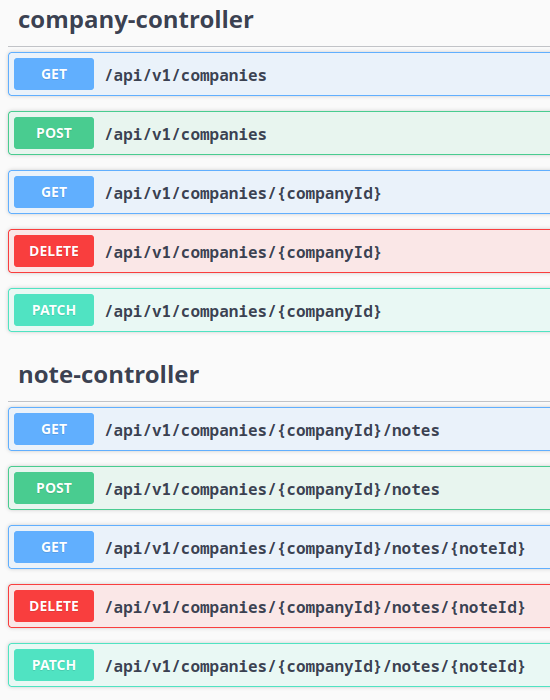
\includegraphics[scale=0.7]{spring_endpoints.png}
				\caption{\label{fig:spring-swagger-endpoints} Spring - endpointy w Swagerze}
			\end{center}
		\end{figure}
		Endpointy do operacji CRUD przygotowane przy pomocy Springa. Company-controller udostępnia standardowe endpointy dla zasobu company. Z kolei note-controller odpowiada za operacje dla zasobu zagnieżdżonego note, który istnieje tylko jako zasób podrzędny względem company.
		
		
		
		\subsubsection{Ruby on Rails}
		Endpointy wygenerowane przy pomocy komendy \cite{RoRDocs}
		\begin{verbatim}
			rails generate scaffold 
		\end{verbatim}
		oraz przygotowaniu zasobu note jako zasobu podrzędnego względem company:
		
		\begin{figure}[H]
			\begin{center}
				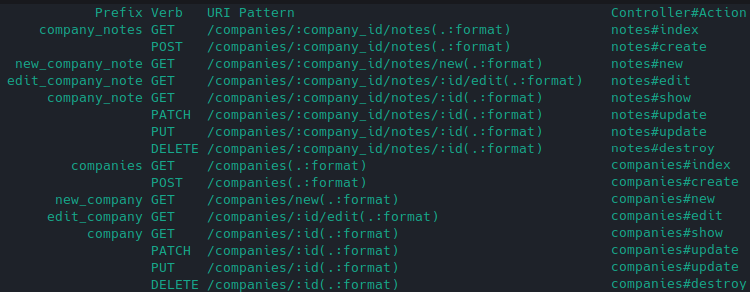
\includegraphics[scale=0.8]{ror_rails_routes.png}
				\caption{\label{fig:ror-endpoints} Ruby on Rails - endpointy}
			\end{center}
		\end{figure}
	
		Jak widać, oprócz podstawowych akcji CRUD Ruby on Rails wygenerował też dwa dodatkowe endpointy, które służą do zwrócenia widoków z formularzami do tworzenia (/companies/new) i akutalizacji (/companies/:id/edit) zasobu company. Warto również zauważyć, że Ruby on Rails dopuszcza metodę PATCH oraz PUT w celu edycji zasobu. Ponadto, do każdego endpointu dodany jest parametr :format, który wskazuje, w jakim formacie danych zostanie zwrócona odpowiedź (obsłużone w kodzie są html oraz json). \\
		
		\noindent Na przykład, dla zapytania:
		\begin{verbatim}
			http://localhost:3000/companies/?format=json
		\end{verbatim}
		zwrócone zostaną dane w formacie json:
		
		\begin{figure}[H]
			\begin{center}
				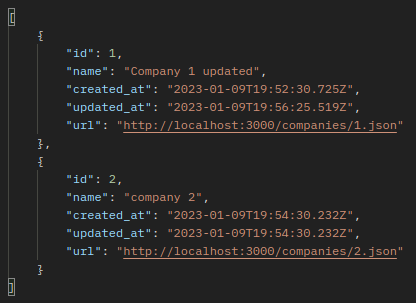
\includegraphics[scale=0.8]{ror_format_json.png}
				\caption{\label{fig:ror-json} Ruby on Rails - odpowiedź json}
			\end{center}
		\end{figure}
	
		
		\noindent Z kolei dla parametru ?format=html zwrócona zostanie zwykła strona html. \\
		
		\noindent Ruby on Rails zwraca również, w odpowiedzi w formacie json, url który po kliknięciu przeniesie użytkownika do konkretnego zasobu.
	
	
	
